% Recompose the twelve unchanged tiles of the accepted raster. Trim amounts
% are pixel fractions of its natural dimensions, independent of image DPI.
\begingroup
\newsavebox{\pcaSourceBox}
\newlength{\pcaSourceWidth}
\newlength{\pcaSourceHeight}
\sbox{\pcaSourceBox}{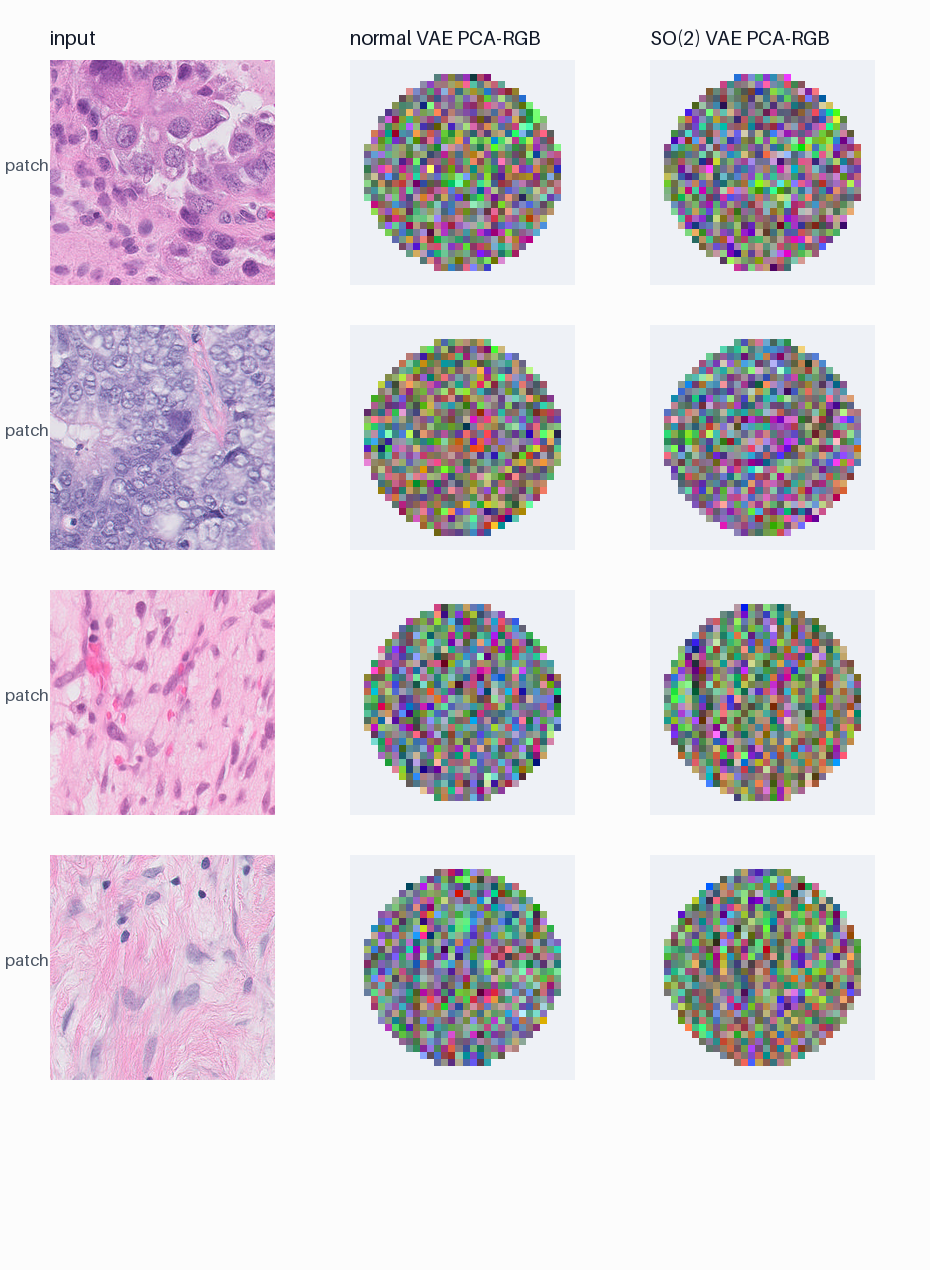
\includegraphics{latent_spatial_pca_maps.png}}
\setlength{\pcaSourceWidth}{\wd\pcaSourceBox}
\setlength{\pcaSourceHeight}{\ht\pcaSourceBox}
% Arguments: left, bottom, right, top margins in the 930 x 1270 raster.
\newcommand{\pcaTile}[4]{%
    \begingroup
    \edef\pcaTrim{%
        \the\dimexpr\pcaSourceWidth*#1/930\relax\space
        \the\dimexpr\pcaSourceHeight*#2/1270\relax\space
        \the\dimexpr\pcaSourceWidth*#3/930\relax\space
        \the\dimexpr\pcaSourceHeight*#4/1270\relax}%
    \edef\pcaGraphic{\noexpand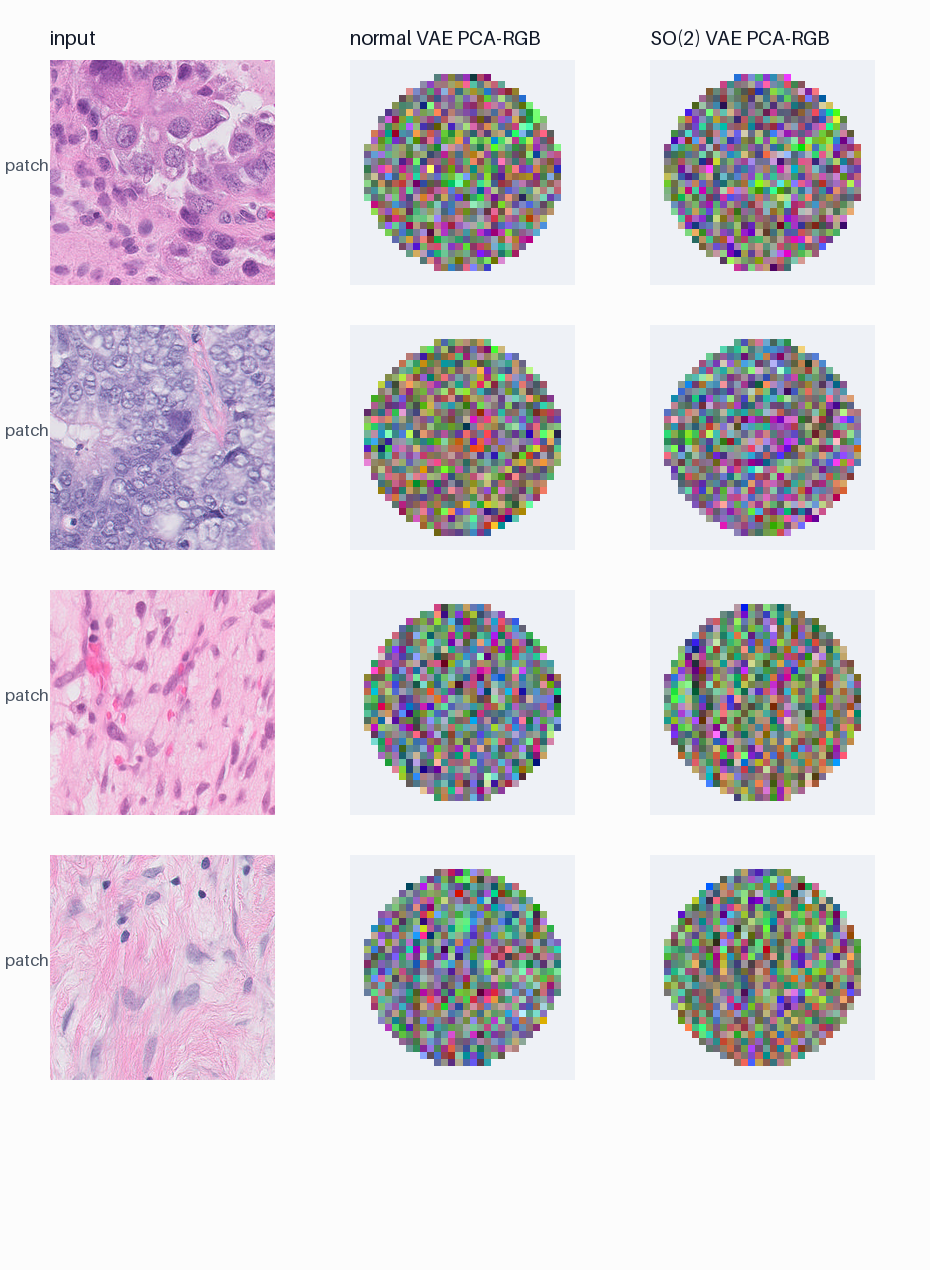
\includegraphics[trim={\pcaTrim},clip,
        width=\noexpand\linewidth]{latent_spatial_pca_maps.png}}%
    \begin{minipage}[c]{0.26\textwidth}
        \pcaGraphic%
    \end{minipage}%
    \endgroup}
\newcommand{\pcaLabel}[1]{%
    \begin{minipage}[c]{0.12\textwidth}
        \centering\sffamily\small\bfseries Parche #1
    \end{minipage}}
\setlength{\tabcolsep}{0pt}
\begin{tabular}{@{}c@{\hspace{0.025\textwidth}}c@{\hspace{0.025\textwidth}}c@{\hspace{0.025\textwidth}}c@{}}
    & \textsf{\small\bfseries Entrada}
    & \textsf{\small\bfseries VAE base}
    & \textsf{\small\bfseries VAE-SO(2)} \\
    \noalign{\vskip 0.15cm}
    \pcaLabel{0} & \pcaTile{50}{985}{655}{60}
        & \pcaTile{350}{985}{355}{60} & \pcaTile{650}{985}{55}{60} \\
    \noalign{\vskip 0.25cm}
    \pcaLabel{8} & \pcaTile{50}{720}{655}{325}
        & \pcaTile{350}{720}{355}{325} & \pcaTile{650}{720}{55}{325} \\
    \noalign{\vskip 0.25cm}
    \pcaLabel{12} & \pcaTile{50}{455}{655}{590}
        & \pcaTile{350}{455}{355}{590} & \pcaTile{650}{455}{55}{590} \\
    \noalign{\vskip 0.25cm}
    \pcaLabel{24} & \pcaTile{50}{190}{655}{855}
        & \pcaTile{350}{190}{355}{855} & \pcaTile{650}{190}{55}{855}
\end{tabular}
\endgroup
